\section{The Taxonomy}\label{sec:taxonomy}

The taxonomy based on the set of documents found in the literature is presented in three parts. The first consists in the taxonomy of \acrshort{CT} applications. The second part covers the communication technologies, both the requirements of the \acrshort{CT} applications and the characteristics of the technologies. The third and last part maps the technologies that can be used for each application. 

\subsection{\acrshort{CT} Applications}

%In this part, we will deal with the results we obtained during our data collection for the Transport part. To do this, it was necessary to distinguish between information disseminated for transport and telecommunications. For example, the specific application requirements (KPI) are intended for the telecommunications part because they are linked to the performance of wireless technologies. On the other hand, the type of road that the application can deploy will be a transport criterion.

This section will cover the various attributes used to differentiate the \acrshort{CT} applications. There are many ways to categorize these applications, in particular with various degrees of detail: for example, how many different vehicle type warning applications or collision risk warning applications should there be? The attributes, in particular the \acrshort{KPI} requirements, are key, as the goal of the taxonomy is to identify possible communication technologies for each application. Similar applications with the same attributes can thus be grouped. 

%To differentiate transport applications, we have chosen several criteria. We asked ourselves how far we should go. For example, for \textit{"Overtaking vehicle warning"} applications, should we differentiate between right and left overtaking applications? If we wanted to do purely transport application taxonomies, we could have separated them. But as for these two applications the requirements (KPI) are identical for its correct functioning, we have decided to merge them into a single application: \textit{"Overtaking vehicle warning"}. Other examples, we wondered, what should we collect or distinguish between apps? For example for the applications \textit{"Across traffic turn collision risk warning"} and \textit{"Merging traffic turn collision risk warning"}, if the applications deal with \textit{"Traffic turn collision risk warning"}, we have considered that communications and messages transmitted during communication are fundamentally different.

Following the information collected in the various documents, all applications were grouped into 61 distinct applications for this taxonomy. All the applications with their acronyms and their definitions are presented in~\ref{appendix:app}. 
The various attributes used to describe the applications are presented in the rest of the section. All attributes are non-exclusive, i.e.\ an application can take several possible values of each attribute. 
%For each specific application, we can issue a definition that is as exhaustive as possible and assign specific attributes to it. These attributes, we can list them in terms of different classes. For example the transport category (safety application or efficiency application) but also other classes such as the roads type or the users types that we will see in the rest of this article.


\subsubsection{Categories}
The first attribute deals with the nature of each application, i.e. the type of use the application will have for transportation or the type of impact the application will have on transportation. Categories include safety, efficiency and the environment. The categories were treated as non-exclusive, with each application possibly attached to several categories: for example, an intersection management application can improve both safety and efficiency. The categories result in a classification of the applications, which can then be analyzed at that level. The categories are also broadly related to their priority, for example safety has a higher priority than other applications in most situations. 

%One of the most relevant elements that we encountered in our reflections and in the articles read was the grouping of the different specific applications in terms of category or even sub-category. We could see that these elements are essential to identify the nature of a specific application, but also to see similarities in terms of requirement for each group of applications. So we will see what type of category we could have:

% {\bf BRUNI: jusqu'ici on a parlé de classes et subclasses. par contre, ci-dessous on parle de catégories. Donc, ça a l'air comme de quelque chose désagregé avec ce qu'on dit au-dessus} 

%{\bf Category}

% In the articles we have read, especially in the articles dealing with the taxonomy of transport applications, that specific applications can be grouped in terms of transport category. These categories make it possible to quickly know the importance and priority of specific applications, for example depending on traffic situations, a safety application will have priority over an infotainment application. But these categories also make it possible to verify the needs, of which we are in the telecommunications part.

Categories were added iteratively as applications were identified, adding new ones as applications did not fit existing ones. 15 categories were identified at the end of the proecess: 

\begin{enumerate}
\item[$A1$] the \textbf{safety} category deals with applications that aim to improve safety, i.e. by drecreasing the risk of a crash~\cite{hamida_security_2015};
  %groups together all the applications which aim to help all transport players (driver, vehicles, infrastructure, etc.) by transferring information on all situations, in particular on dangerous situations such as accidents \cite{hamida_security_2015}
\item[$A2$] the \textbf{efficiency} category deals with applications that aim to improve traffic by avoiding lost time and stops through data collection and sharing, and optimal vehicle control~\cite{hamida_security_2015};
  %collecting the different positions and statuses of transport players. 
\item[$A3$] the \textbf{entertainment} category covers the applications that provide users with access to the internet and media for their entertainment~\cite{hamida_security_2015};
  % gathers the applications which make it possible to transmit an access to multiple data to the user, in particular with the access to Internet. Which allows users to have fun or work 
\item[$A4$] the \textbf{confort} category includes the applications that aim to increase the comfort of road users~\cite{hamida_security_2015};
\item[$A5$] the \textbf{security} category includes the applications that aim to make road users more secure, e.g.\ to avoid the theft of a vehicle or to intervene in case of an emergency (other than for a crash); 
\item[$A6$] the \textbf{parking} category deals with applications that aim to help a driver park one's vehicle; 
\item[$A7$] the \textbf{environnement} category deals with application that aim to decrease the environmental impacts of transportation~\cite{chang_estimated_2015};
\item[$A8$] the \textbf{data collection} category relates to applications that collect data about any of the component of the transportation systems, vehicles, the infrastructure or users;   
\item[$A9$] the \textbf{freight} category deals with applications for freight (the movement of goods);
\item[$A10$] the \textbf{energy} category covers applications that aim to manage energy consumption, without an explicit goal to decrease the potential environmental impacts;
\item[$A11$] the \textbf{vehicle maintenance} category covers applications that aim to help with vehicle maintenance;
\item[$A12$] the \textbf{economic} category deals with applications that support the purchase of transportation services, economic activity and other economic aspects of transportation;
  % cost of transportation or to support the economy through the movement of people and goods;
\item[$A13$] the \textbf{access} category deals with applications that manage the access of users or vehicles to specific roads or zones; 
\item[$A14$] the \textbf{shared transport} category includes applications to share vehicles or manage fleets of vehicles;
\item[$A15$] the \textbf{traveler information} category deals with applications that provide useful information to users about their trips.
\end{enumerate}

Since an application can belong to several categories, the relationship between applications and categories is many-to-many. For example, a \emph{Speed Limit} application relates to safety, efficiency, the environment and energy. Such a relationship can be naturally represented as a bypartite graph or a Sankey diagram, as done in Figure~\ref{fig:app-category}.

It should be noted that some documents used sub-categories, for example of the different types of safety applications, but that most generally put each application in only one category. The sub-categories were not retained for this taxonomy for two reasons. The main was that sub-categories were not relevant for the telecommunication technologies: applications in the same sub-category generally had the same \acrshort{KPI} requirements. Second, sub-categories appeared often arbitrary and did not exist for all categories. 

%{\bf Sub-Catgory}

%The presence of transport subcategories was mentioned in the various articles studied and was the subject of reflection for the construction of the taxonomy. These subcategories correspond to categories within the categories formulated above. For example, a safety application can be classified in a subcategory of the type: Collossion application, road hazard warning application / road sign notification ect . 
%This classification in terms of transport has a certain logic because it allows to separate and atomize the applications for more specific research. But since the taxonomy relates to the requirements of specific applications, it was noted that the subcategories do not differentiate applications in terms of telecommunications. For example, for safety applications, the message sizes are similar, but totally different for infotainment applications. 
%It is with this type of reflection that on the one hand the classifications of the sub-categories have not been taken into account, but also to facilitate the understanding of the taxonomy. 

\begin{figure}[ht!]
  \begin{center}
    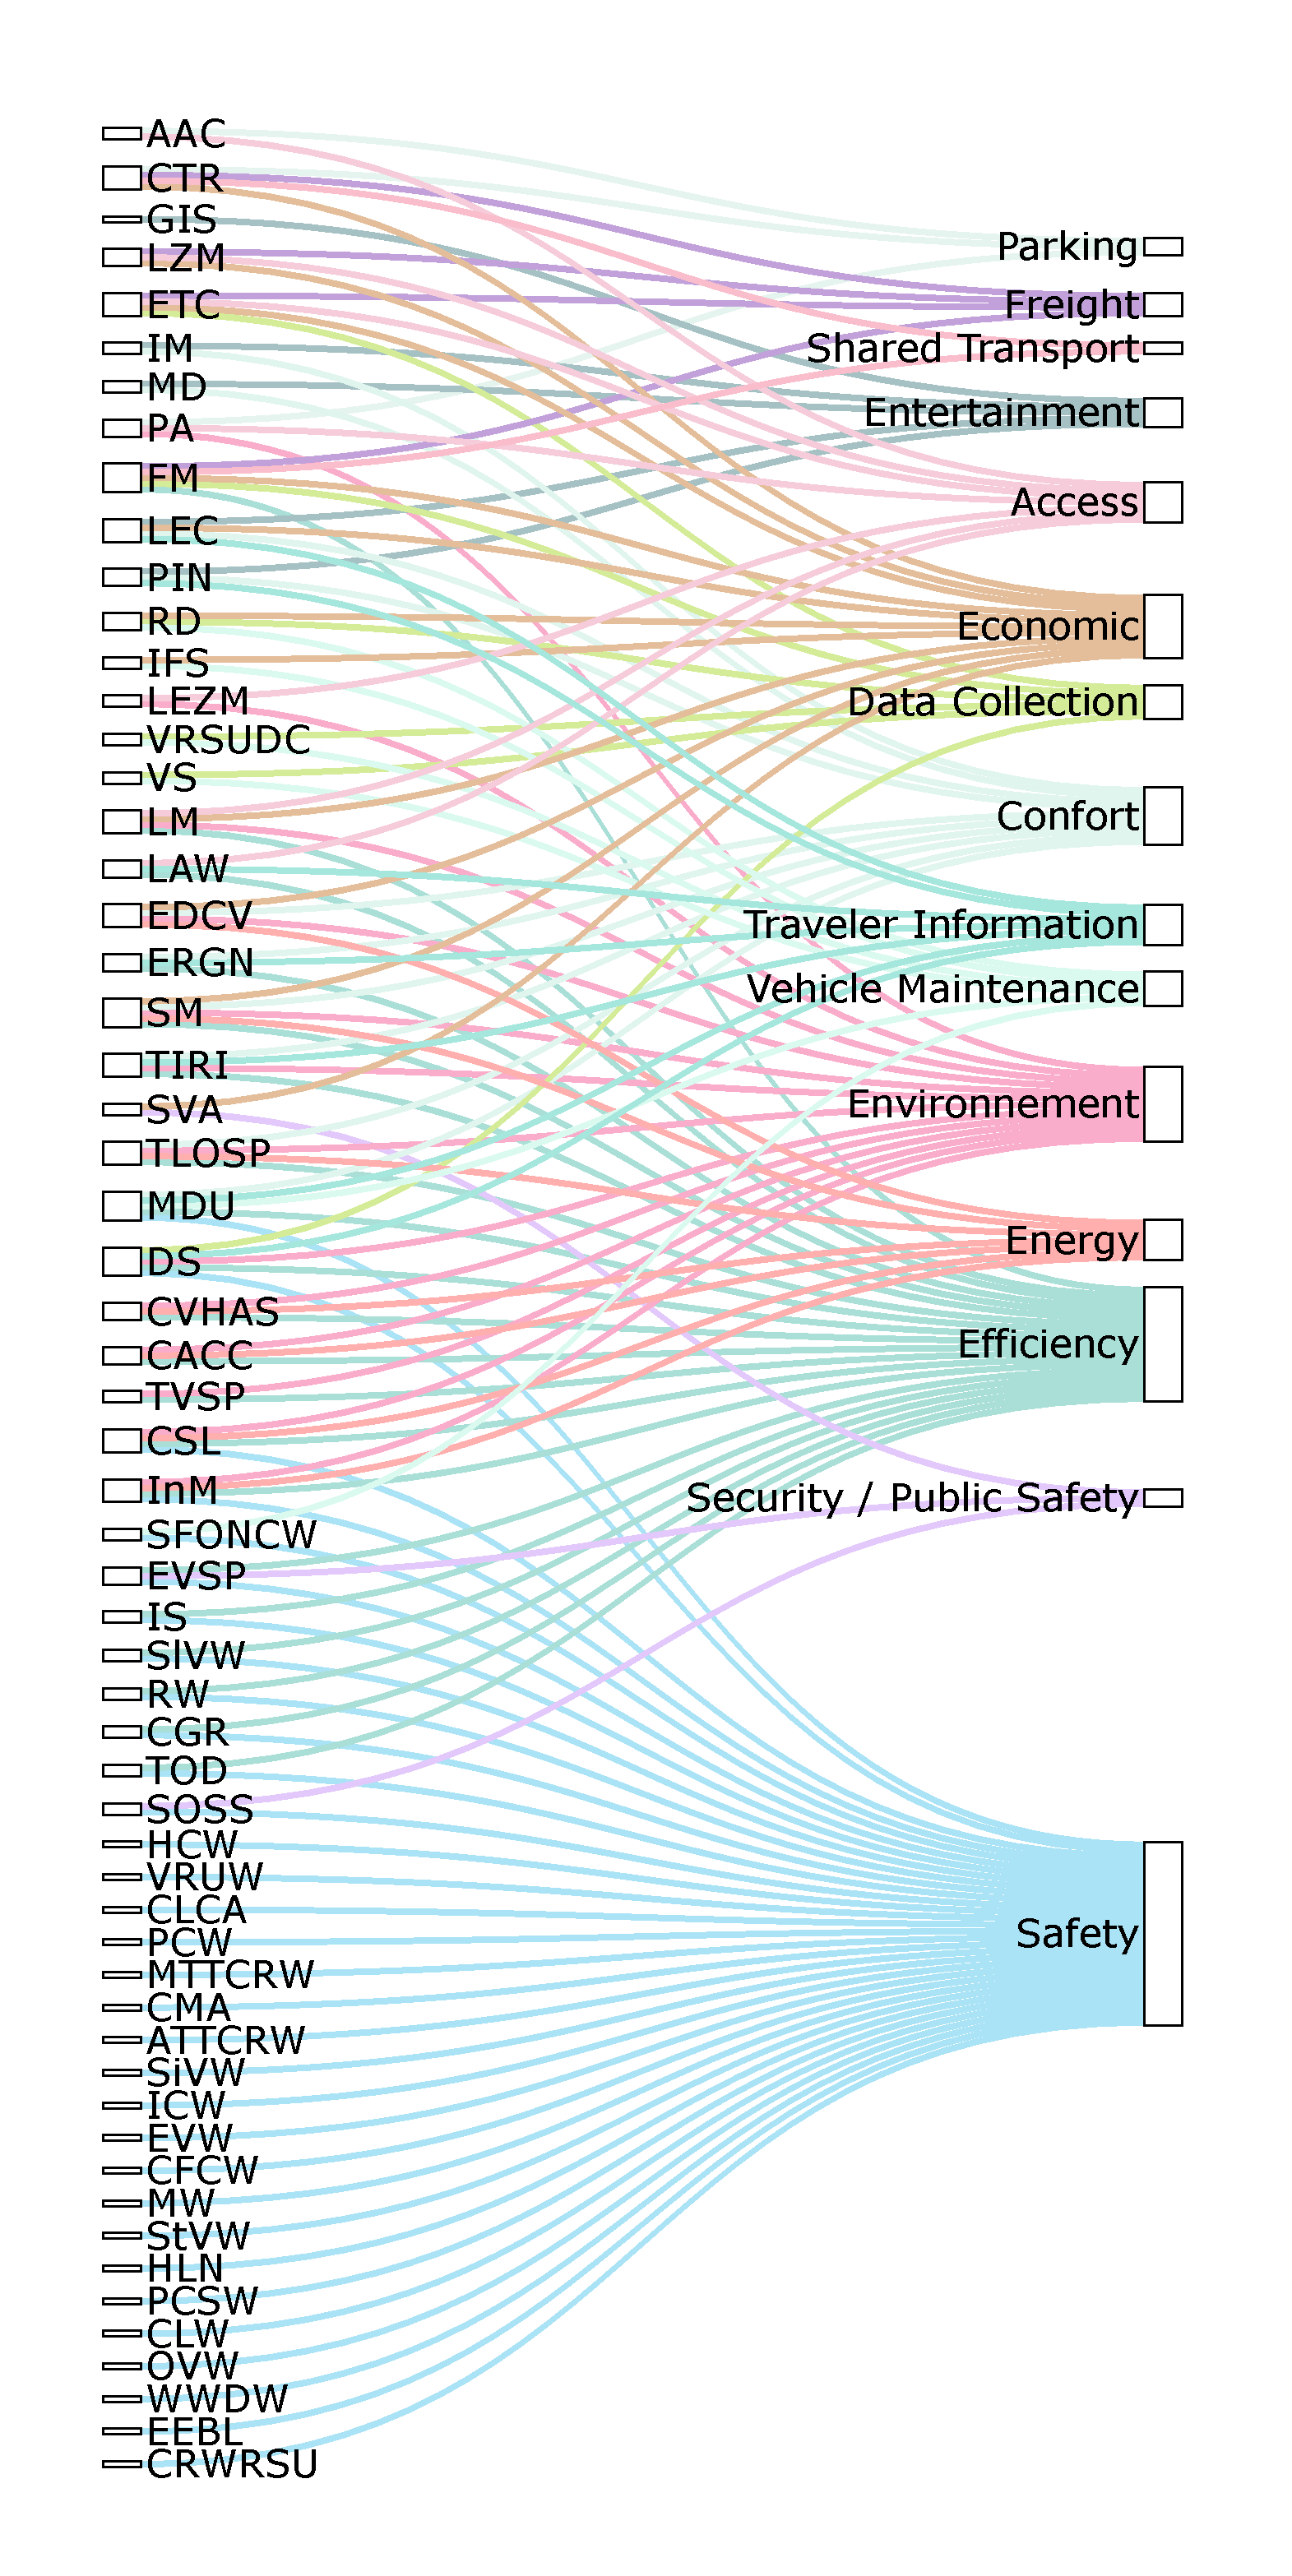
\includegraphics[width=0.7\textwidth]{category_sankey.pdf}
    \caption{Illustration of the application categories (see section~\ref{appendix:app} for the acronyms).}
    \label{fig:app-category}
  \end{center}
\end{figure}
%\FloatBarrier

\subsubsection{User Types}
The next attribute is the type of road user that may be involved in the use of the application or receive information or a warning from it.
% This attribute is obviously related to the mode of communication, e.g.\ vehicle to vehicle (V2V), vehicle to infrastructure (V2I) and vehicle to pedestrian (V2P).
Deciding which type of road user is involved is not always easy, as the main user of most applications is a driver of a passenger car or a commercial vehicle. The possible user types are listed below:

% Another useful classification is to focus on the type of user involved in each specific application. This type of classification has many advantages, it makes it possible to see which user is involved in the transport on the one hand and on the other hand it makes it possible to identify whattype of communication mode may be involved. For example if a specific application affects a vehicle and a pedestrian, we can expect the application to be V2P, even if the application implies that a vehicle is a transport provider, we can expect an application of type V2I. 

\begin{enumerate}
\item[$U1$] \textbf{Driver}: this category includes motorcyclists, commercial vehicle and public transit drivers; 
  % This category corresponds to people who drive or not a motorized vehicle on the road. These vehicles can range from cars to simple bikes
\item[$U2$] \textbf{Passenger};
  % Corresponds to people who move passively, that is to say who are not the driver of the vehicle transporting it.
\item[$U3$] \textbf{Pedestrian};
  % Corresponds to the person who does not use material means to move around
\item[$U4$] \textbf{Cyclist};
\item[$U5$] \textbf{Motorcyclist};
\item[$U6$] \textbf{Public Transit Driver};
\item[$U7$] \textbf{Commercial Vehicle Driver}.
  % Public or private entity that offers transport services, such as public transport for example. Actors indirectly linked to the mobility of the driver, who offers offers adapted to the user who wants or who travels and influences his movements. These could be, for example, parking lot operators
\end{enumerate}

Motorcyclists, commercial vehicle and public transport drivers are selected when an application specifically targets them. All applications with the driver attribute are relevant for all drivers, regardless of the specific vehicle. 
% The relationship between the applications and road user types is shown in a Sankey diagrame in Figure~\ref{fig:user_by_app}.
The number of applications per road user types is shown in Figure~\ref{fig:nb-app-attribut}. 

\begin{figure}[ht!]
  \begin{center}
    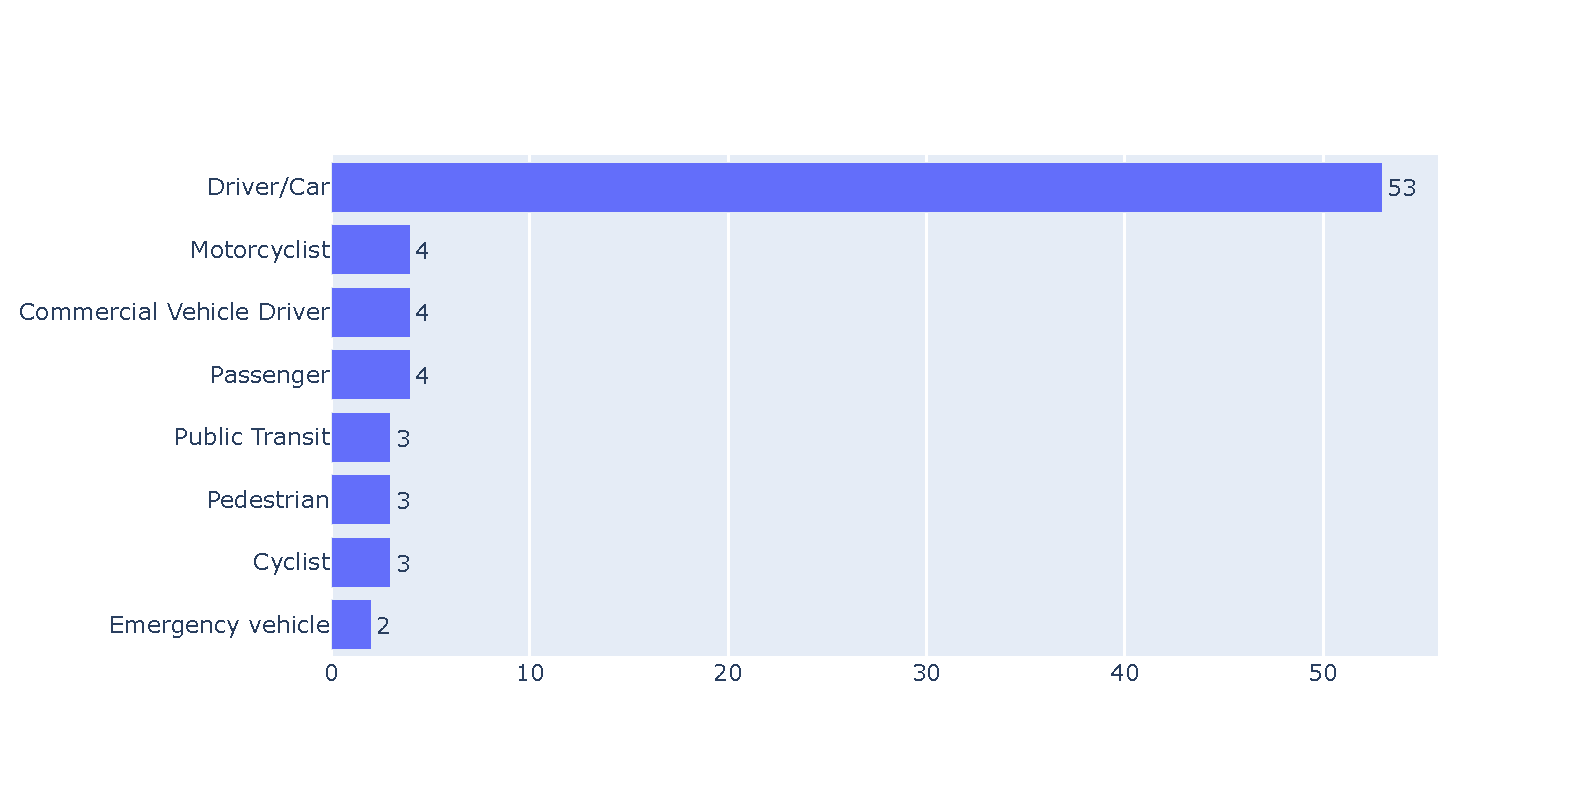
\includegraphics[width=0.5\textwidth]{diagramme_bar_attribut/user_types.pdf}\\
    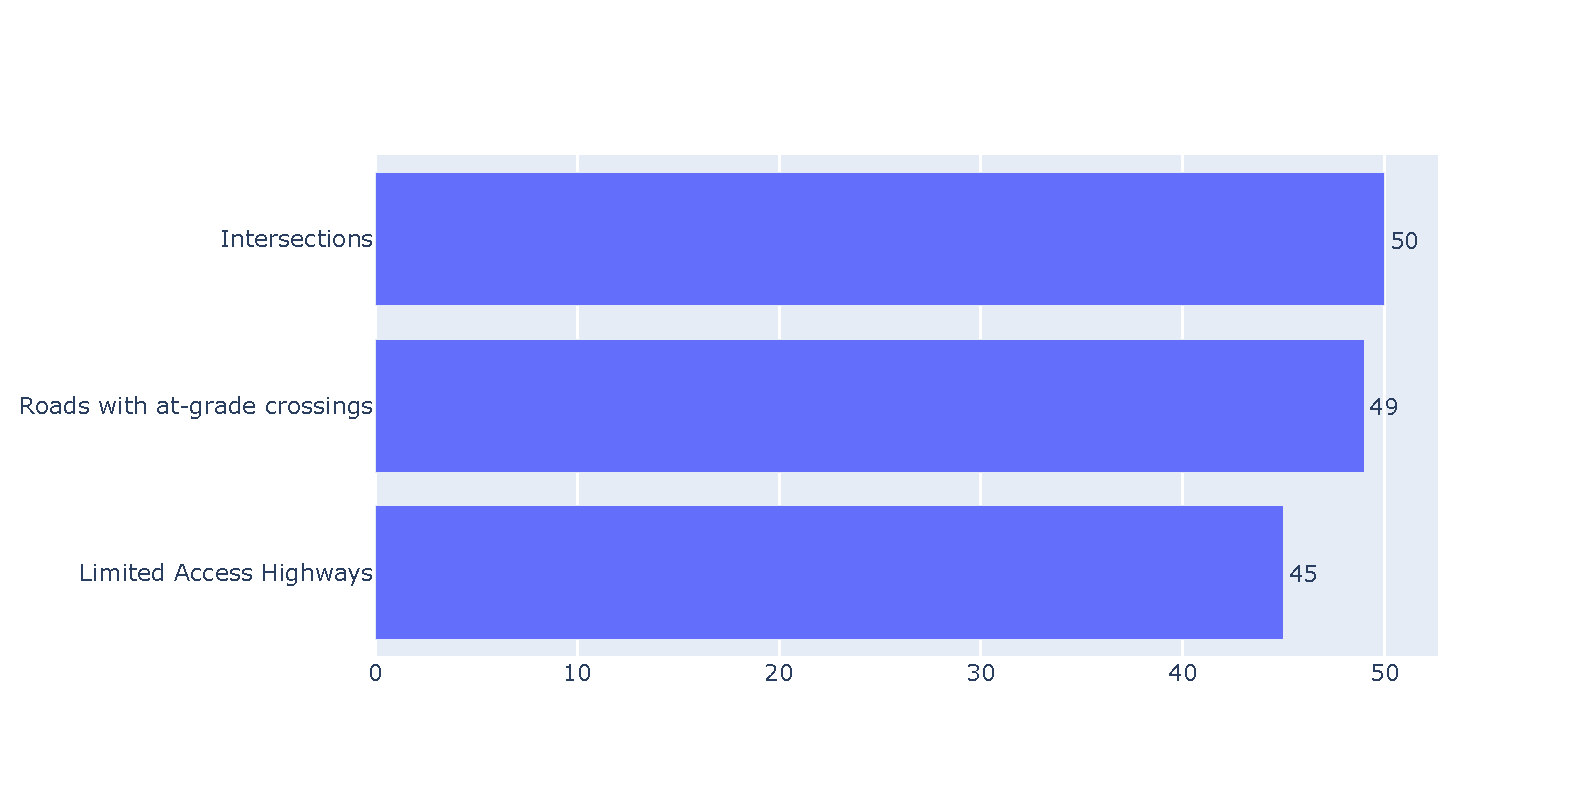
\includegraphics[width=0.495\textwidth]{diagramme_bar_attribut/road_types.pdf}
    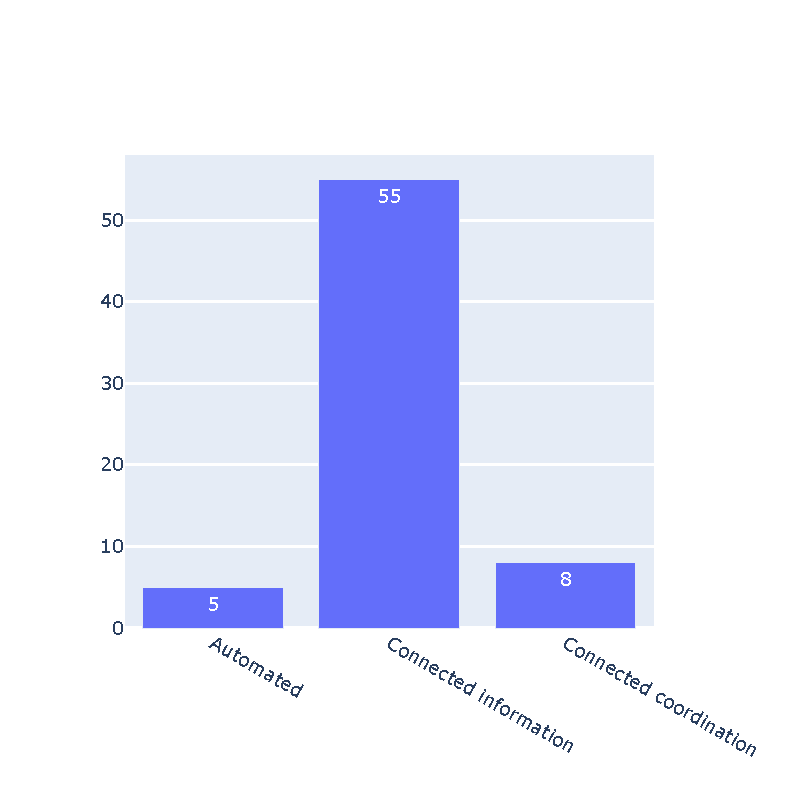
\includegraphics[width=0.495\textwidth]{diagramme_bar_attribut/mechanisms.pdf}
    \caption{Distribution of the number of applications according to road user types (top), road types (bottom left) and application mechanisms (bottom right).}
    \label{fig:nb-app-attribut}
  \end{center}
\end{figure}


\subsubsection{Road Type}
% Regarding transport, we can classify the different applications according to different criteria, we have seen that it is possible to do this in terms of transport categories and in terms of user type. Another class which is interesting and makes it possible to distinguish the type of road taken into account for the good implementation of specific transport applications.
Another important attribute relates to the parts of the networks where each application exclusively or typically operates. There are qualitative differences in the type of traffic on road segments and at intersections, and whether the intersections on a segment are at grade or not. This is related to the first two functions of roads, access and transit, which are inversely correlated: the more access to adjacent properties a road provides, the less important the transit function of the road, implying lower speeds. 
The following types of roads or parts of the network are considered:

%This type of classification has several effects, first of all we can assign road types to each application, for example applications of the type "Traffic light optimal speed advisory" cannot in theory be taken in roads Limits Access Highways on the other hand in the Intersections it can be integrated. The other effects come from the deployment of technologies that we will see in the rest of the article. Indeed, depending on the type of road, the type of infrastructure may be different and therefore the type of wireless technologies may be different. 


\begin{enumerate}
\item[$R1$] {\bf Limited access highways} are roads without any access to adjacent properties and no at-grade intersections. On such roads, one can move at high speeds without having to stop at intersections: traffic can be continuous (uninterrupted) as the only hindrance is other road users;% High speed road with few or no intersections 
\item[$R2$] On {\bf roads with at-grade intersections}, vehicles may have to stop at intersections, e.g.\ controlled by traffic control devices such as stop signs and traffic lights, and also for other modes of transportation such as public transportation and walking: such traffic is called discontinuous;
  % provides more access
  % Moderate speed road with at grade corssings
\item[$R3$] {\bf Intersections} of roads or with infrastructure for other modes of transportation are the most complex part of a road network, involving issues of safety and efficiency that traffic and priority rules attempt to address. %Low speed road with intersections like traffic light
\end{enumerate}

As can be seen in Figure~\ref{fig:nb-app-attribut}, most applications apply to all these road types, but some are only relevant to one, e.g.\ to intersections in the case of traffic lights, or to roads with at-grade intersections in the cases where the application requires access to adjacent property, which is not possible on limited access highways. 


\subsubsection{Application Mechanisms}
The last attribute is the mechanism by which the application has the desired effect. Connectivity between vehicles, users and pieces of infrastructure let them exchange data and information, which can be used in different ways, most importantly to inform the driver for him to make decision and take action, or to let the vehicle in some cases take action in an automated way. The application mechanism is thus categorized as:

%A last classification in connection with the telecommunications part and which is for us a category which will take more and more place in future research of communication transport applications, is the classification of application mechanisms. This category concerns automation and the nature of the information transmitted between each type of user. To do this, we can distinguish two types of information (and decision) transmitted in the applications:

\begin{enumerate}
\item[$AM1$] {\bf Connected information}: such applications provide data and information obtained through communication with other vehicles, users and pieces of infrastructure to the driver who has the control of the vehicle: this implies that the driver can ignore the information of the \acrshort{CT} application;
  %This type of information takes into account the information transmitted by a vehicle or an infrastructure to other traffic users without any cooperation in decisions. This is the case, for example, with the \textit{"Pre-Crash sensing Warning"} application where information is transmitted on unavoidable accidents but the information will be taken without taking into account the condition of other road users.
\item[$AM2$] {\bf Connected coordination}: such applications not only exchange information between vehicles, users and infractructure, but also let the vehicles coordinate to find a solution that is better for all users than any solution that could have been found if each user decided separately;\\
  a good example is ``Co-operative adaptative cruise control'' where users can coordinate to select the optimal braking rate to avoid a crash and optimize other impacts such as energy consumption;
  % This type of information is a special case of connected information. In this case, we classify the applications where information and decision-making are done collectively in a coordinated manner between users. For example, in the case of platoon-type applications, vehicles will collectively make decisions to optimize their speed and other elements.
\item[$AM1$] {\bf Automated}: such applications use the data and information they receive to directly control at least one function of the a vehicle such as acceleration or braking. 
\end{enumerate}

This attribute is important for the efficiency of the applications, as coordinated or automated applications will be more effective than what the driver may do based on the provided information. It is also related to some communication \acrshort{KPI}s as coordination will require more data exchanges for the vehicles to make a decision collectively. It should be noted that applications that support infotainments services, \acrfull{GIS}, \acrfull{IM} and \acrfull{MD} do not correspond to any of the above categories. From the number of applications per mechanism types shown in Figure~\ref{fig:nb-app-attribut}, it is obvious that the vast majority of \acrshort{CT} applications only provide information to the driver. 

%As for the categories of transport, the choice of the representation of the road types was a sankey  Fig  \ref{fig:application_mecanisme}

\subsection{Telecommunication Technologies}
%After having seen all the useful classifications for the transport part for the different specific applications, we will focus on the telecommunications part. 
%To do this, focusing on the objective of the article, if possible, note the requirements of specific applications and assimilate to each specific application the wireless technologies that can be used.
%To do this, we will do two studies in this part of telecommunications, first we will focus on current wireless technologies that take into account their performance and secondly we will focus on the requirement of each specific application. 
The first step is to define the main \acrshort{KPI}s used to describe the \acrshort{CT} application requirements and the telecommunication technology capabilities. Second, the wireless telecommunication technologies that may be used in \acrshort{CT} applications are listed. They are often discussed in the literature under the topic of vehicular ad hoc networks (VANET). These technologies fall into three categories: short (below 100~m), medium (between 100~m and 1~km) and long range (above 1~km)~\cite{anwer_survey_2014,shree_novel_2016}. 
The characteristics of the different technologies are presented in each category. 
The last step is to present the modes of communications related to the components of the transportation networks involved in the various transportation applications. 
Figure~\ref{fig:wireless_techs} depicts the wireless technologies in terms of transmission range and data rate.

\begin{figure}[ht!]
  \begin{center}
    \includegraphics[width=0.5\textwidth]{../image/wireless_technologies.jpg}
    \caption{Communication technologies as a function of range and data rate. {\bf NS: refaire en pdf}}
    \label{fig:wireless_techs}
  \end{center}
\end{figure}

\subsubsection{Telecommunication and Application KPIs}

%In this part, we will now focus on the telecommunications aspect for specific applications, that is to say the sufficient criteria for the proper functioning of the latter. To do this, like the technologies, we will separate two studies, first we will look at the KPIs of the applications and secondly we will analyze the modes of communication deployed for these specific transport applications. 

\acrshort{KPI}s may be qualitative or quantative. There are many \acrshort{KPI}s used in the literature and not all are relevant for this taxonomy. In particular, all the \acrshort{KPI}s that allow to link the requirements of \acrshort{CT} applications to the performance of communication technologies were kept. They are defined in the following list in terms of requirements for the functioning of the applications:
%There is a lot of information in the articles about the different specific applications, so it is important to choose the KPIs that are useful for our studies. We therefore decided to take the 

\begin{enumerate}
\item the {\bf latency} is the maximum duration allowed to carry out the communication~\cite{etsi_etsi_tr_102_638_intelligent_2009}; %  for the proper functioning of the application
\item the {\bf range} is the minimum distance at which information should be transmitted between the users, vehicles and units involved;
\item the {\bf message frequency} is the number of messages transmitted by the application per unit of time;
\item the {\bf message size} is the size of the message transmitted during the communication; {\bf NS: size up or just size?}
\item the {\bf data rate} is the minimum rate of data transmitted during the communication of the application; %It is often expressed in bits/s
\item the {\bf priority} represents the relative importance of messages across different applications. For example, security messages take priority over infotainment messages. There are three levels: high, medium and low; 
\item the {\bf message type} is the nature of the message transmitted, for example whether it is periodic or not. 
\end{enumerate}

When not available, the data rate is derived as the product of the message size mutiplied by the message frequency. The communication technologies are described with a few attributes, namely the relevant standard, frequency and bandwidths, and the following extra \acrshort{KPI}s:

\begin{enumerate}
\item signal interference;
\item accessibility;
\item security.
\end{enumerate}
% Standard & Data Rate & Range & Latency & Signal Interference  & Frequency & Bandwidths & Accessibility & Security

{\bf NS: definir ces KPIs\\
Brunilde, a relire les definitions (des KPIs ci-dessus et des technologies ci-dessous)}

It should be noted that the deployment of some technologies, namely the technologies forming cellular networks like 5G and LTE, is expected to be dense to cover most transportation facilities in such a way that the application range criterion will be met, independently of the communication technology intrinsic range (if it was sparsely deployed). 


%For an easier to understand representation of this article, a grouping of KPIs by category has been favored, as shown in the figure at parallel coordinates.


\subsubsection{Descriptions and Categories of Communication Technologies}
%In this part, we will list the different wireless technologies used in our study to build the taxonomy. To do this, we tried to take all the technologies that use the different modes of communication included in our taxonomy (V2V, V2I, V2P).
%In the literature, these technologies are often linked to the implementation of the ad hoc network of vehicles (VANET), which seemed relevant to our study. 
%Thus, after compilation of the data, we were able to take charge of categories of technologies according to their transmission range:

\paragraph{Short Range Communication Technologies}\ \\
Short range communication technologies, sometimes referred to as short-region wireless technologies~\cite{yu_technology_2018}, refer to technologies that communicate in a small region of the order of a maximum of 100~m. These types of technologies are more suitable for indoor applications as well as outdoor applications that require small distances between the equipments. Their \acrshort{KPI}s are presented in Table~\ref{tab:short-range-com}.
% and a minimum level of the order of a millimeter.

\begin{table}[ht!]
  \centering
  \caption{Short Range Communication Technology \acrshort{KPI}s}
  \label{tab:short-range-com}
  \begin{tabular}{p{1,4cm} p{1cm} p{1cm} p{1cm} p{1cm} p{1.5cm} p{1.2cm} p{1.3cm} p{1.4cm} p{1.4cm}}
    \hline
    Technology & Standard & Data Rate & Range & Latency & Signal Interference  & Frequency & Bandwidths & Accessibility & Security\\
    \hline
    UWB &  IEEE 802.15.3  & 480 Mb/s	&   10 m - 75 m	 &  0.1 ms  & Low & 3.1-10.6 GHz	 &500 MHz - 7.5 GHz	 & Contention based	& High\\
   
    Bluetooth  & IEEE 802.15.1	& 1-24 Mb/s	&  10 m&	100 ms  & High &  2.4 GHz	& 1 MHz& 	Schedule Based	& Low\\
	
    BLE  & IEEE 802.15.1	& 1 Mb/S	&  50 m& 6 ms & High&	2.4 GH &	2 MHz 	&Schedule Based&	Low\\

    ZigBee& IEEE 802.15.4	&20-250 Kb/s&	 100 m	&30 ms  &High	&868 MHz, 902–968 MHz and 2,4GHz	&2 MHz & Schedule Based	&High\\
    \hline
  \end{tabular}
\end{table}

\textbf{\acrfull{UWB}} is a technology belonging to the IEEE 802.15.3 standard which operates on a frequency band between 3.1 and 10.6~GHz and for a bandwidth between 500~MHz and 7.5~GHz~\cite{anwer_survey_2014,ahangar_survey_2021}. Being short range, this technology can send data up to 10~m for its best performance and up to 75~m with a minimum latency of 0.1~ms~\cite{ahangar_survey_2021}. Its highest data rate corresponds to 480~Mb/s~\cite{wang_networking_2019}. The advantage of UWB over most other short range technologies is that it experiences little interference during communication and is therefore ideal for dense areas and meetings in crowded places~\cite{ahangar_survey_2021}. 

\textbf{Bluetooth} technologies belong to the IEEE 802.15.1 standard which operates on a frequency band of 2.4~GHz and for a bandwidth of 1~MHz~\cite{anwer_survey_2014,ahangar_survey_2021}. Like UWB technologies, its range is around 10~m but with a low data rate of only around 1 to 24~Mb/s with a latency of 100~ms~\cite{ahangar_survey_2021}. While the advantage of Bluetooth is that it is present in our environment and is relatively inexpensive to deploy, it only connects two entities at a time and has very strong interference, which prevents from functioning well in very busy environments~\cite{wang_networking_2019,bluetooth_bluetooth_2021,akpakwu_survey_2018}. 

\textbf{\acrfull{BLE}} is a version of Bluetooth that consumes less energy while keeping the same performances remain except for the range up to 50~m with lower latency (6~ms). The advantage of course is that this technology consumes less energy but it is not compatible with the other Bluetooth standard that is very common in our environment~\cite{ahangar_survey_2021}. 

The \textbf{ZigBee} technology follows the IEEE 802.15.4 standard that uses different frequency bands like 868~MHz, 908-968Mhz~and 24~Ghz, for a bandwidth of 2~MHz~\cite{ahangar_survey_2021}. The advantages of this technology are the range of 100~m and the latency of 30~ms. However, the data rate is only 250~Kbps, making it a convenient technology for applications requiring small message sizes, regardless of the fact that this technology is susceptible to interference~\cite{anwer_survey_2014,ahangar_survey_2021,shree_novel_2016,selvarajah_zigbee_2008}. 

%\textbf{InfraRed}


\paragraph{Medium Range Communication Technologies}\ \\

\begin{table}[ht!]
  \centering
  \caption{Medium Range Communication Technologies \acrshort{KPI}s}
  \label{tab:medium-range-com}
  \begin{tabular}{p{1,4cm} p{1cm} p{1cm} p{1cm} p{1cm} p{1.5cm} p{1.2cm} p{1.3cm} p{1.4cm} p{1.4cm}}
    \hline
    Technology & Standard & Data Rate & Range  & Latency & Signal Interference  & Frequency &  Bandwidth & Accessibility & Security\\
    \hline
    Wi-Fi &  IEEE 802.11n  &  54 Mb/s	&   240 m &  50 ms  & High & 2.4-5 GHZ	 & 20 MHz	 & Contention based&	Low\\
    
    DSRC / Wave  & IEEE 802.11p	& 27 Mb/s	& 1 km&	100 ms  & Low &  5.9 GHz	& 10 MHz& 	Contention based &	High\\
    \hline	
  \end{tabular}
\end{table}

Communication technologies are most often classified in short and long range technologies. In our case, we decided to add a third category: medium range communication technologies with a range between 100~m and 1~km. Their \acrshort{KPI}s are presented in Table~\ref{tab:medium-range-com}.%Here are the technologies that we took in our study:

\textbf{\acrfull{Wi-Fi}} technologies follow the IEEE 802.11 standard. Its transmission range (250~m) sometimes puts it in the category of short range technologies~\cite{araniti_lte_2013,anwer_survey_2014}. This technology uses two frequency bands, 2.4~GHz and 5.2~GHz, with a channel bandwidth between 1~and 40~Mhz~\cite{papadimitratos_vehicular_2009}, has a low latency of 50~ms and a maximum throughput of 54~Mb/s~\cite{ahangar_survey_2021}. However, due to high interference with its communication environment, Wi-Fi seems difficult to be deployed for high density applications~\cite{chen_lte-v_2016}.

The \textbf{\acrfull{DSRC}} is based on IEEE 802.11p and is used both for \acrshort{V2V} and \acrshort{V2I} communications~\cite{ahangar_survey_2021}. This technology uses the 5.9~GHz frequency band with a 10~MHz bandwidth~\cite{ghosal_security_2020}. 
Its maximum range of 1~km with a data rate of 27Mb/s puts it in the medium range category~\cite{anwer_survey_2014}. It has a latency of 100~ms~\cite{ahangar_survey_2021}. Its advantages are its medium range, low latency and low interference, ideal for security applications. However, this type of technology is limited in the event of heavy congestion~\cite{cailean_survey_2014}. Wireless access in vehicular environments (WAVE) is considered along \acrshort{DSRC} because these technologies are almost identical, except for the physical layer~\cite{ghosal_security_2020}.

\paragraph{Long Range Communication Technologies}\ \\

\begin{table}[ht!]
  \centering
  \caption{Long Range Communication Technologies \acrshort{KPI}s}
  \label{tab:long-range-com}
  \begin{tabular}{p{1,4cm} p{1cm} p{1cm} p{1cm} p{1cm} p{1.5cm} p{1.2cm} p{1.3cm} p{1.4cm} p{1.4cm}}
    \hline
    Technology & Standard & Data Rate & Range  & Latency & Signal Interference  & Frequency & Bandwidth(s) & Accessibility & Security\\
    \hline
    Wi-Max &  IEEE 802.16m &100 Mb/s	& 15 km&  10 ms  & High & 2.5, 3.5, 5.8 GHz	 & 5, 10, 20MHz & Schedule Based&	High\\
    
    LTE-4G & 3GPP &1 Gb/s	&  11 km &  50 ms  & Low & 2-5 GHz	 &  5, 10, 15, 20 MHz	 &Contention based&	High\\
  
    5G - Low-band & 3GPP &250 Mb/s	&  15 km &  30 ms  & Low & < 1GHz	 &  800-1900 MHz	 &Contention based&	High\\
  
    5G - Mid-band & 3GPP &900 Mb/s	&  1 km &  10-20 ms  & Low & 60 GHz	 &  100 MHz	 &Contention based&	High\\

    5G - mmWave & 3GPP &20 Gb/s	&  100 m &  1 ms  & Low & > 24 GHz	 &  400 MHz	 &Contention based&	High\\

    NBIoT & 3GPP &200 Kb/s	&  10 Km &  50 ms  & Low &  2.4 GHz	 &  200 KHz	 &Contention based&	High\\

    MBWA & IEEE 802.20 &4.5 Mb/s	&  15 km &10ms & High & 3.5 GHZ 	 & 5, 10, 20 MHz  	 &Schedule Based&	High\\

    MicroWave & IEEE 802.15.4 &16 Gb/s	&  10 km &   & High & 	 &  	 &Contention based&	Low\\

    LoRa  &801.15.4g&50 Kb/s	&  5-15 km & 400 ms  & Low & 865 - 923 MHz	 & 125, 250, 500 Khz 	 & Contention based&High	\\

    SigFox  &3D-UNB &100 b/s - 600 b/s	&  10-50 km & 1s  & Low & 25 MHz - 1 GHz	 &  192KHz &Contention based&High	\\
   
    DASH7  &D7A &167 kb/s&  1 km &   &  & 433, 868/915 MHz	 &  25 kHz or 200 kHz	 &Schedule Based& High	\\

    Ingenu-RPMA  & IEEE 802.15.4k&624 kb/s&  45km &   &  & 2.4 GHz	 & 1 MHz 	 &&High	\\
    \hline
  \end{tabular}
\end{table}

Compared with the other communication technologies, the long range category contains technologies with a range greater than 1~km. Their \acrshort{KPI}s are presented in Table~\ref{tab:long-range-com}.

The \textbf{\acrfull{WiMax}} technology complies with the IEEE 802.16m standard and uses the 2.5~GHz frequency band. This long range technology can communicate up to 15~km~\cite{selvarani_comparative_2014} and transmit at a speed of 100~Mb/s~\cite{anwer_survey_2014} in the case of mobile transmission~\cite{selvarani_comparative_2014} with a latency of 10~ms~\cite{msadaa_comparative_2010}. The advantage of this technology is that it has a very large transmission range.

{\bf Hugues: Comme pour la 5G, verifier les valeurs des technologies}

The \textbf{\acrfull{LTE}} and \textbf{\acrfull{LTE-A}} technologies developed by 3GPP and marketed under the names 4G use a frequency band of 2~GHz~\cite{seo_lte_2016} and a bandwith that can go up to 100~MhZ~\cite{araniti_lte_2013}. %By separating 5G, the deployment capacity
The range can reach 11~km~\cite{shah_5g_2018} with a transmission of 1~Gb/s~\cite{araniti_lte_2013} and a low latency of 10~ms, which make this technology appropriate for all applications. 
%For simplicity and to avoid taking the less obsolete technologies, LTE-A includes LTE

The \textbf{5G} technology follows the 3GPP standard and is the latest version of mobile technologies about to be deployed in many cities. The latter is eagerly awaited for its performance and is expected to speed up the implementation of ITS applications~\cite{foubert_long-range_2020}. Unlike 4G, 5G could be deployed in three frequency bands: a low-frequency band (less than 2~GHz), a mid-frequency band (between 3~GHz and 6~GHz, often called sub-6~GHz band) and a high-frequency band (above 24~GHz, often called millimeter wave (mmWave))~\cite{foubert_long-range_2020}. 5G is intended to provide high data rate reaching 20~Gb/s~\cite{hussain_integration_2019}.
In addition, with this improved performance, a latency of less than 1~ms is expected~\cite{hussain_integration_2019} and a range between a few hundred meters and more than 10~km~\cite{foubert_long-range_2020}. This promising technology could address several shortcomings of current technologies, especially for security applications that use \acrshort{DSRC}~\cite{shah_5g_2018}. 

\textbf{\acrfull{NBIoT}} is a \acrfull{LPWAN} technology proposed by 3GPP for low cost, low battery life and \acrfull{C-IoT} applications~\cite{qadir_low_2018,routray_narrowband_2021}.

The \textbf{\acrfull{MBWA}} technologies follow the IEEE 802.20 standard, use the 3.5~GHz frequency band, and exchange at a data rate of 4.5~Mb/s in a communication area of 15~km \cite{anwer_survey_2014}.

% \textbf{MicroWave}

\textbf{\acrfull{LoRa}} uses different frequency bands depending on the continent, e.g.\ for the USA 915~MHz and 433~MHz~\cite{li_lora_2018}. Its deployment is different depending on the environment, going from 5~km in urban areas, up to 15~km in rural areas, with exchange rate at a speed of 50~kb/s~\cite{foubert_long-range_2020, queralta_comparative_2019} and a high latency (400~ms)~\cite{potsch_towards_2019}. This promising technology is a very low-cost solution, yet not feasible for latency sensitive applications given its high latency.

\textbf{SigFox} has a low data rate (100 to 600~bp/s) and a long range (10~km in urban areas and up to 50~km in rural areas)~\cite{potsch_towards_2019}. This technology uses a frequency band of 869 and 915~MHz and consumes very little energy~\cite{akpakwu_survey_2018}. Despite a large deployment, it would be difficult to use for \acrshort{CT} applications given the low data rate. 

The \textbf{DASH7} technology uses 433~MHz as the frequency band, at a low rate of 197~kb/s~\cite{akpakwu_survey_2018}. Unlike other long-range technologies, it has a range of 1~km in urban areas
% , which makes it a medium-range technology
, but is less efficient than \acrshort{DSRC}~\cite{foubert_long-range_2020}.

The \textbf{Ingenu-RPMA} technology is compliant with IEEE 802.15.4k standard~\cite{akpakwu_survey_2018} and uses the 2.4~GHz frequency band~\cite{foubert_long-range_2020}. 
Its range can reach 15~km in an urban environment, but it has a data rate of only 156~kb/s~\cite{foubert_long-range_2020} which makes it difficult to use for \acrshort{CT} applications. %to set up as part of a communication application}.

%We have just seen in this categorization the definitions of wireless technologies and their performance as a general telecommunication tool. But an important piece of information is in what type of communication mode can we use these technologies to be able to map them to each specific application requirements. 

\subsubsection{Modes of Communication}
% https://en.wikipedia.org/wiki/Vehicle-to-everything % vehicular communication systems
 
There are various types or modes of communication between the various components of the transportation system, generally centered on the vehicle communicating with a specific type or several types of road users~\cite{araniti_lte_2013,molina-masegosa_lte-v_2017,shladover_connected_2018,dar_wireless_2010,abboud_interworking_2016,chen_lte-v_2016}: 

%Connected cars can communicate in different modes, depending on the transmission and reception ways.. 
%Thus, we can take data to collect useful information on the deployment of technologies in communication modes, for example if a technology can be used in V2I communication 
%In general, the communication mode can be classified as follow:
% In our study, we decided to take into account only 3 types of communication: 

\begin{enumerate}
\item[$M1$] \acrfull{V2V} communications refers to vehicle-to-vehicle communications, without  the use of the telecommunications infrastructure;
  % In \acrfull{V2V} communications,  information are  exchanged directly between motor vehicles without the use of the telecommunications infrastructure. 
\item[$M2$] \acrfull{V2I} communications refer to vehicle-to-infrastructure communications, with various pieces of infrastructure like traffic controllers or sensors are equiped with communication modules that can connect to nearby vehicles;
% In \acrfull{V2I} communications , information are exchanged  between the vehicles and the telecommunications infrastructures. 
\item[$M3$] \acrfull{V2P} communications refer to vehicle-to-pedestrian communications, including pedestrians with mobility devices and cyclists. 
%In  \acrfull{V2P} communications , information are exchanged   between motorized vehicles and non-motorized vehicles such as pedestrians or bicycles. 
\item[$M4$] \acrfull{V2X} communications refer to two or more of the previous communications modes.
\end{enumerate}

\begin{figure}[ht!]
  \centering
  \begin{tikzpicture}[every text node part/.style={align=center}, thick, scale=1.5]
    \node[label={\small V2I}] (un) at(2.3,0){\includegraphics[width=.1\textwidth]{infra.png}};
    \node[label={\small V2V}]  (deux) at (0.8,-3){\includegraphics[width=.1\textwidth]{car.png}};
    \node (trois) at (2.3,-1.5){\includegraphics[width=.1\textwidth]{car.png}};
    \node[label={\small V2P}]  (quatre) at (3.8,-3){\includegraphics[width=.1\textwidth]{pedestrian.png}};
               
    \draw[<->,draw=green!70!red!50,fill=green!5,line width=0.2mm] (trois.north) -- (un.south);
    \draw[<->,draw=blue!90!black!70,fill=green!5,line width=0.2mm] (trois.south west) -- (deux.north east);
    \draw[<->,draw=red!70,fill=green!5,line width=0.2mm] (trois.south east) -- (quatre.north west);
  \end{tikzpicture}
  \caption{Communication Mode}
  \label{fig:com-mode}
\end{figure}

\acrshort{V2X} communications are not explicitly considered in our taxonomy: they can be inferred when a technology supports at least two of the other modes. 
%In our classification of communication modes, we did not consider V2X communication. For us, Vehicle-to-Any (V2X) communication is a communication that combines all previous communications. We therefore noted that if a technology was V2X, it could communicate with all the elements of the environment.
For example, 5G is a technology supporting the V2X communication mode, as it can be deployed for V2V, V2I and V2P applications. 
Some more specific modes of communication have not been taken into account, in particular because they are mostly redundant with the others or not relevant. For example, \acrfull{V2T}~\cite{vandung_nguyen_efficient_2016} and vehicle-to-bycicle/cyclist (V2C) are special cases of \acrshort{V2I} and \acrshort{V2P} communications respectively. 
% We have deliberately not taken into account certain modes of communication, whether it is poor appearance in our applications or redandance in other modes of communication. This is the case of \acrfull{V2T}\cite{vandung_nguyen_efficient_2016} which is, for us alone, a specific case of V2I, but also of Vehciule-to-bycicle, which is a special case of V2P.
% Following the example of the study of technologies, we research for each application which mode of communication is used.

% \begin{figure}[ht!]
%   \begin{center}
%     \includegraphics[width=16cm]{tech.png}
%     \caption{Modes of communication supported by each technology.}
%     \label{fig:mode-com-tech}
%   \end{center}
% \end{figure}
% \begin{figure}[ht!]
%   \begin{center}
%     \includegraphics[width=0.8\textwidth]{communication.png}
%     \caption{Modes of communication supported required by each application.}
%     \label{fig:mode-com-app}
% \end{center}
% \end{figure}

\begin{figure}[ht!]
  \begin{center}
    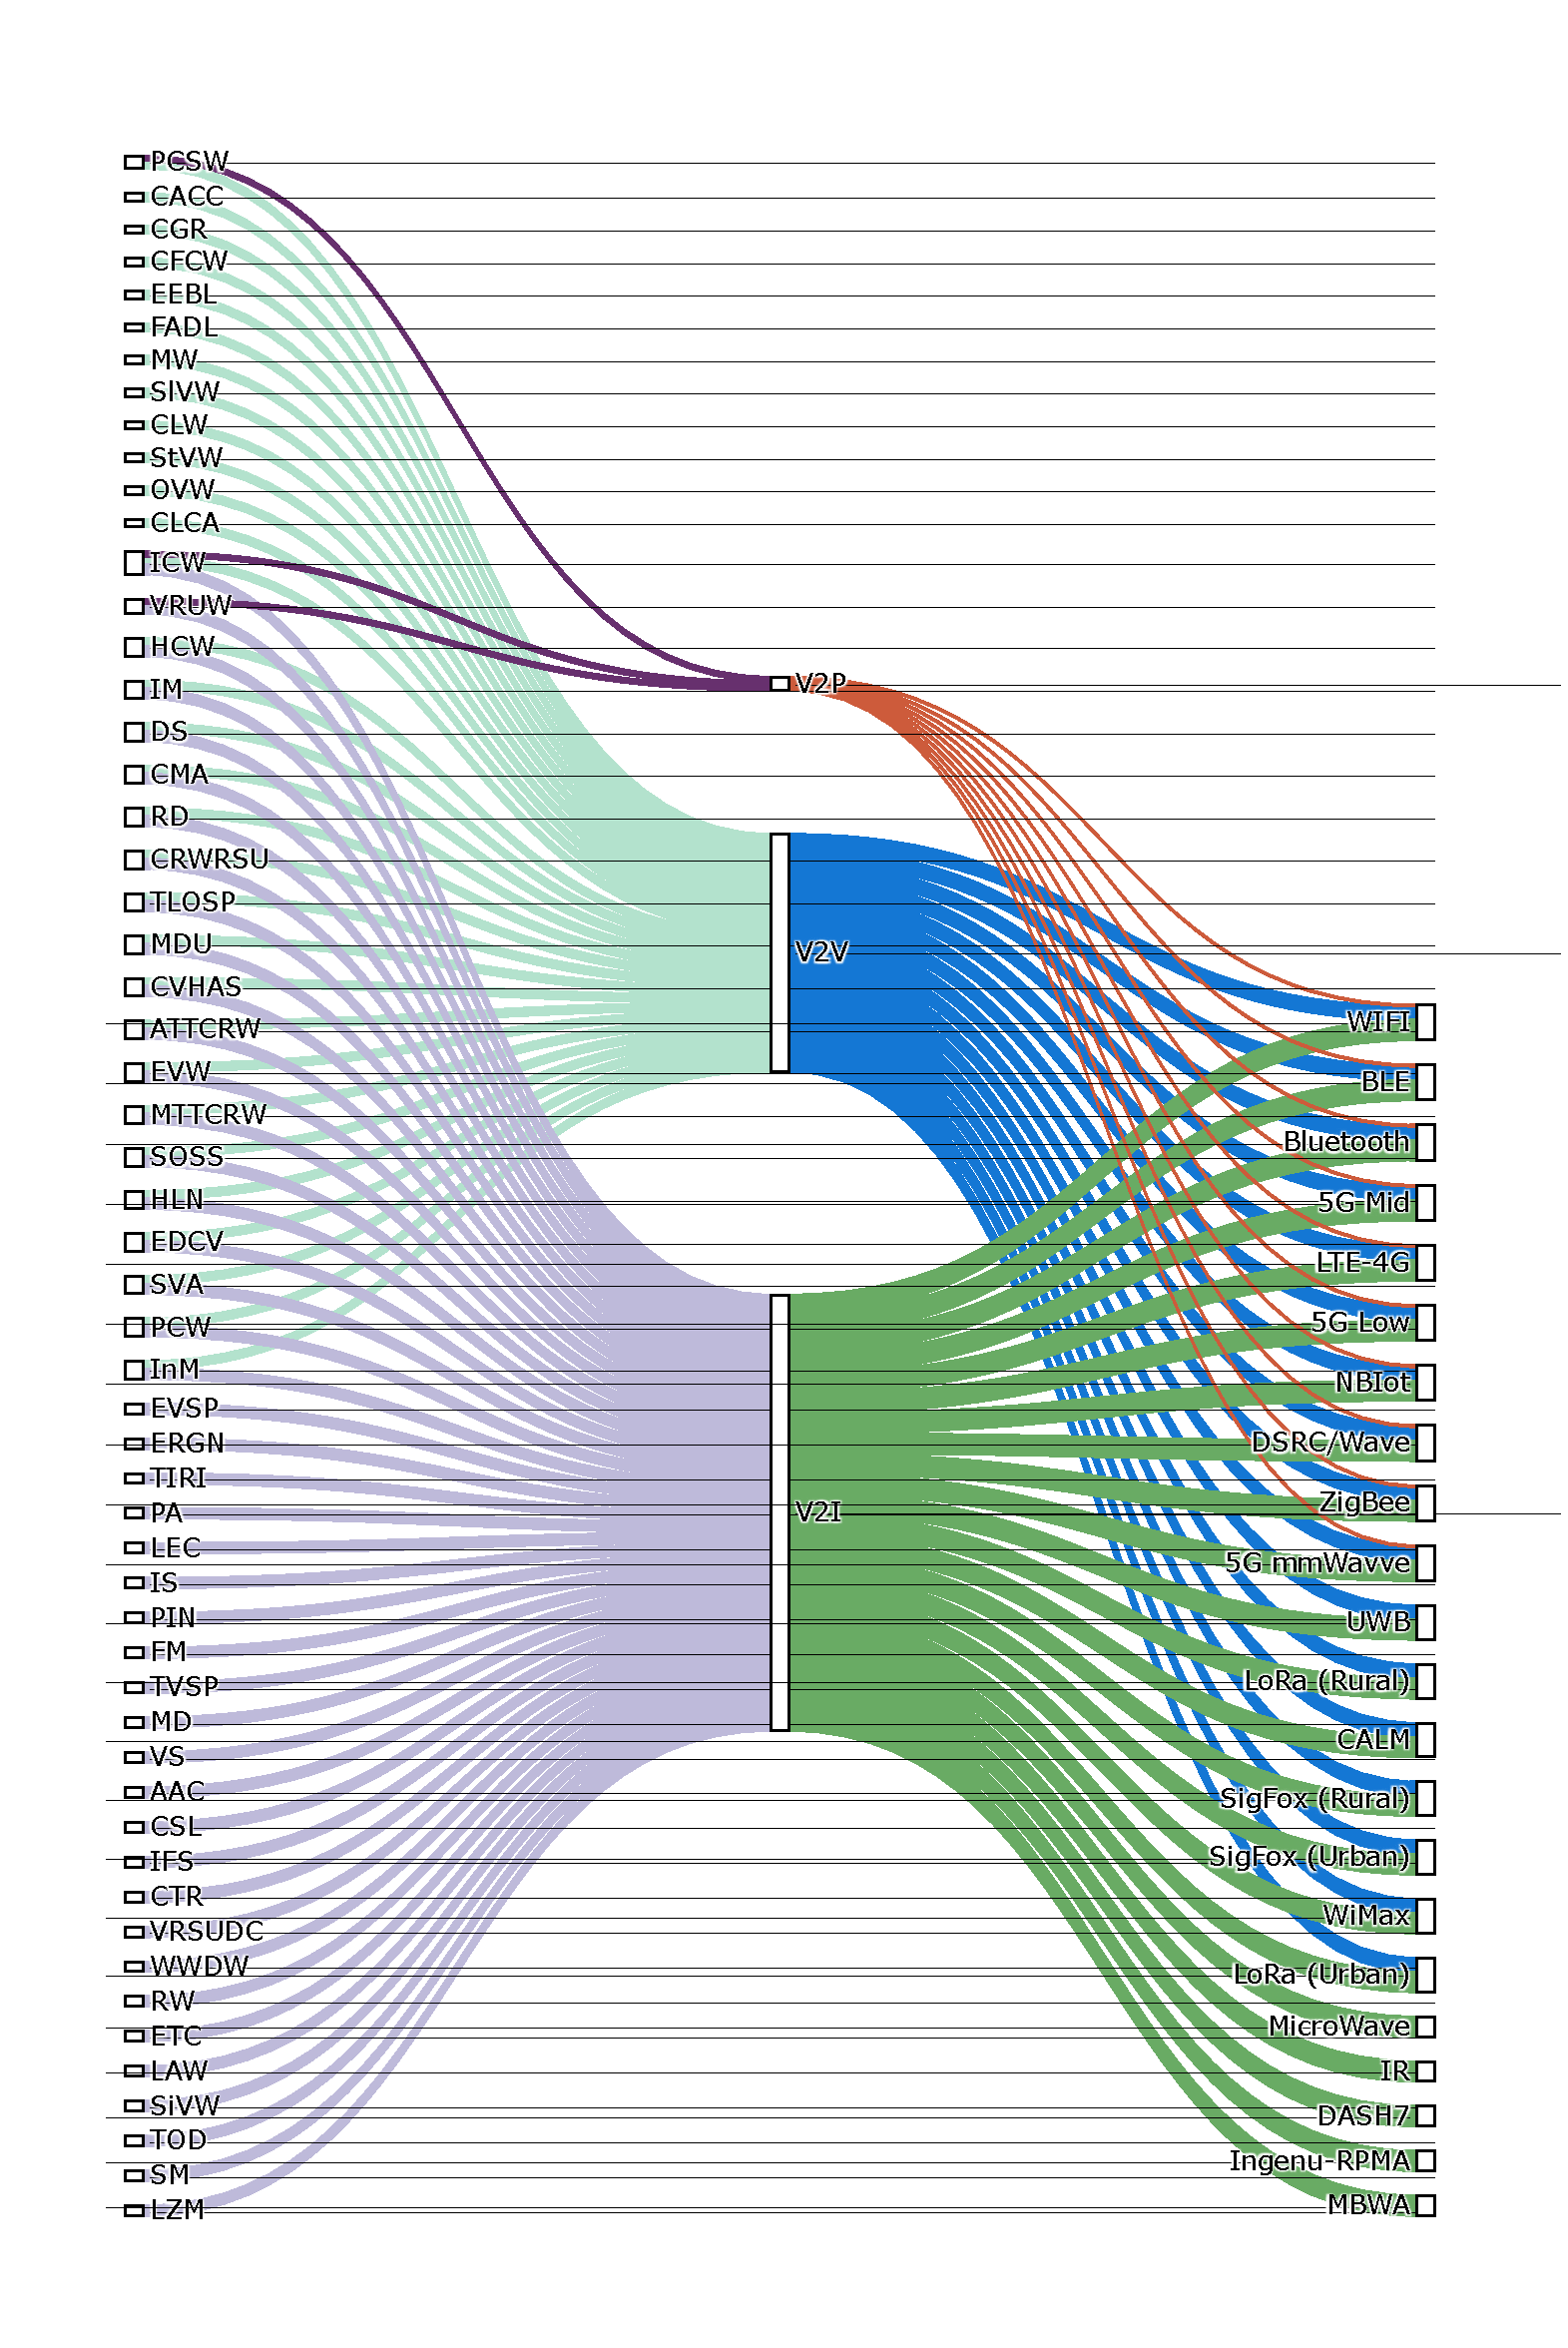
\includegraphics[width=0.9\textwidth]{merge_com_app_tech.pdf}
    \caption{Modes of communication supported by each technology and required by each application}
    \label{fig:fusion_comm}
  \end{center}
\end{figure}

The communication mode used for the operation of each application was generally found in the literature~\cite{hobert_enhancements_2015}. When this information was not readily available, it was derived from the types of road users involved by the application. 
% One of the solutions is to refer to the classification of user types which was mentioned in the transport section.
For example, for the \acrfull{VRUW} application, the \acrshort{V2P} mode is necessary. %We can also cite the pre-crash alert application which will promote V2V communication. This part first tells us about the nature of the application, namely how the application works and how the vehicle communicates in this situation. In two stages, this part allows us to acquire essential information for the last part on the merger of specific application and technologies uselable. So for all applicatin, we can represent communication mode with a Sankey on Figure~\ref{fig:fusion_comm}. 
On the other side, each communication technology can support one or more modes of communication, depending for example on the availability of devices supporting the technology for the elements of the transportation system. Finally, the applications and communication technologies can be linked as illustrated in a Sankey diagram in Figure~\ref{fig:fusion_comm}. 


\subsection{Mapping CT Applications with Communicating Technologies}

In this last section, several \acrshort{KPI}s are analyzed in order to identify the telecommunication technologies deemed to satisfy the requirements of each \acrshort{CT} applications. Not all \acrshort{KPI}s are critical and some could not be used because of a lack of information for the requirements of several applications. The mode of communication is first used to verify the suitability of communication technologies, as can be visualized in Figure~\ref{fig:fusion_comm}.  
The main \acrshort{KPI}s are latency, data rate and range. Range applies for all technologies, except for communication technologies with a dense deployment in the case of V2I communications.
% \acrshort{V2V} and \acrshort{V2I} communication modes.

%communication tech should provide data transmission with max latency, requires some amount of data transmission and to reach vehicles at least x meters away

%In this part, we are going to merge the two modes, that is to say merge the information of the communicating applications in the field of transport that we have visualized in the previous parts with the telecommunication information. This part will eventually make it possible to assimilate to each application one or more technologies that can be used for the proper functioning of this first. 

%{\bf NS: clarifier les critères utilisés pour mapper les applications et les technologies de communication, d'abord selon le mode de communications, puis quels KPI sont utilisés\\ ajouter les deux graphiques du nombre d'applications possibles par catégorie d'application et du nombre d'applications pour lequel chaque technologie peut être utilisé (segmenté par catégorie si lisible)  (2nd graphique à faire)}

%\subsubsection{Merging of modes of communication }
%In the previous section, a study to identify the modes of communication, depending on the wireless technologies and specific applications, was carried out. The first step was therefore to join this telecommunications and transport information. To evaluate applications, a Sankey can be taken into account, as in Figure~\ref{fig:fusion_comm}.

%For example, applications that only use V2P communication to operate will not consider DASH7 technologies for their operation. For example with the application of electronic emergency brake lights (EEBL), the communication is V2V vehicle type, UWB technology is unlikely to be foldable. This classification makes it possible to assign potentially usable technologies to each specific application. However, in view of this information does not take into account the performance of technologies and application requirements for proper operation. 

%{\bf HB: Clarification du mapping }
%To create the mapping, it was chosen to compare specific criteria for specific technologies and applications. The first filtering criterion is based on the mode of communication and on the range of technologies and types of application. Indeed, if the application uses V2I communications, the coverage depends on the position of the base station which is fixed and therefore no filtering is necessary for these applications. Or if the communication is V2V or V2P, the base stations are mobile so if an application needs to communicate messages to other points at a distance x, the technology must be a range y greater than X. The second filters is effects on latency, i.e. whether a technology has enough time to communicate with its environment. And the last filter was based on the data rate, which is the ability of a technology to transmit a message over a period of time. Sometimes the literature gives us this information, under it has been developed by dimensional analysis namely:

% \begin{equation}
% Data\_Rate=Message\_Frequency*Message\_Size
% \end{equation}

\begin{figure}[ht!]
  \begin{center}
    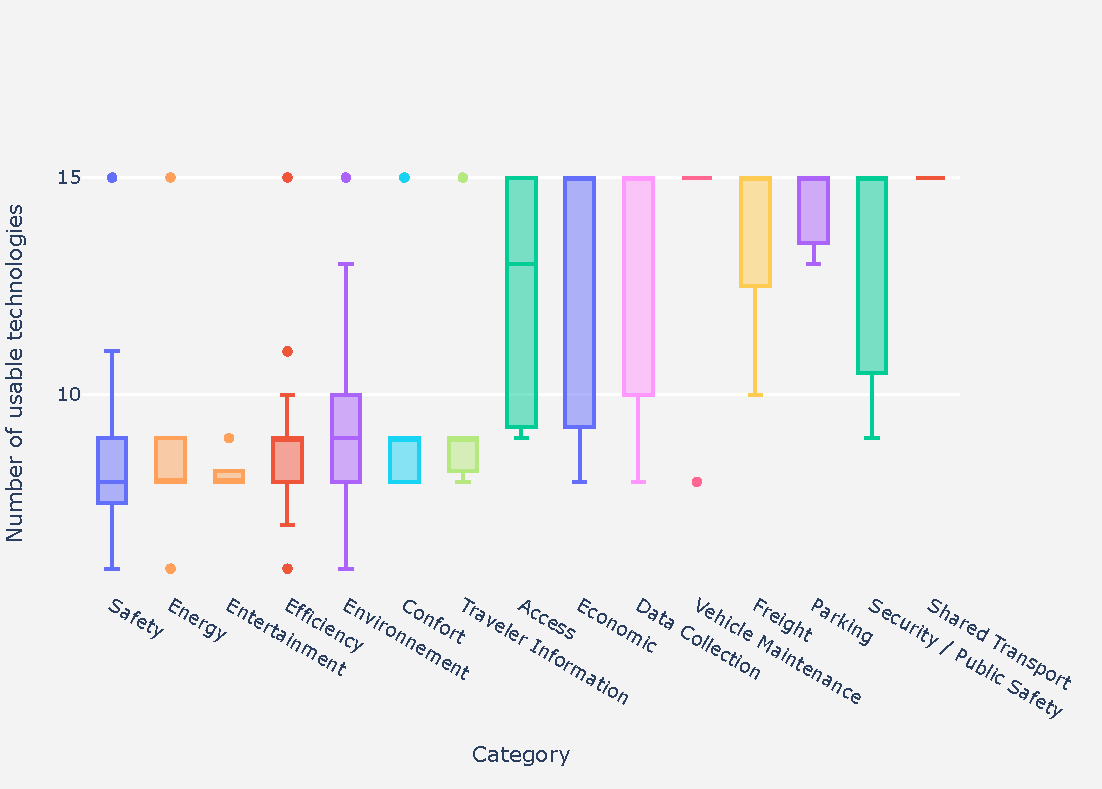
\includegraphics[width=0.9\textwidth]{box_plot.pdf}
    \caption{Distribution of the number of technologies usable by category (the boxplots show the quartiles, as well as the numbers lying outside the whiskers extending beyond the first and last quartile by 1.5 times the interquartile range).}
    \label{fig:boxplot}
  \end{center}
\end{figure}

\begin{figure}[ht!]
  \begin{center}
    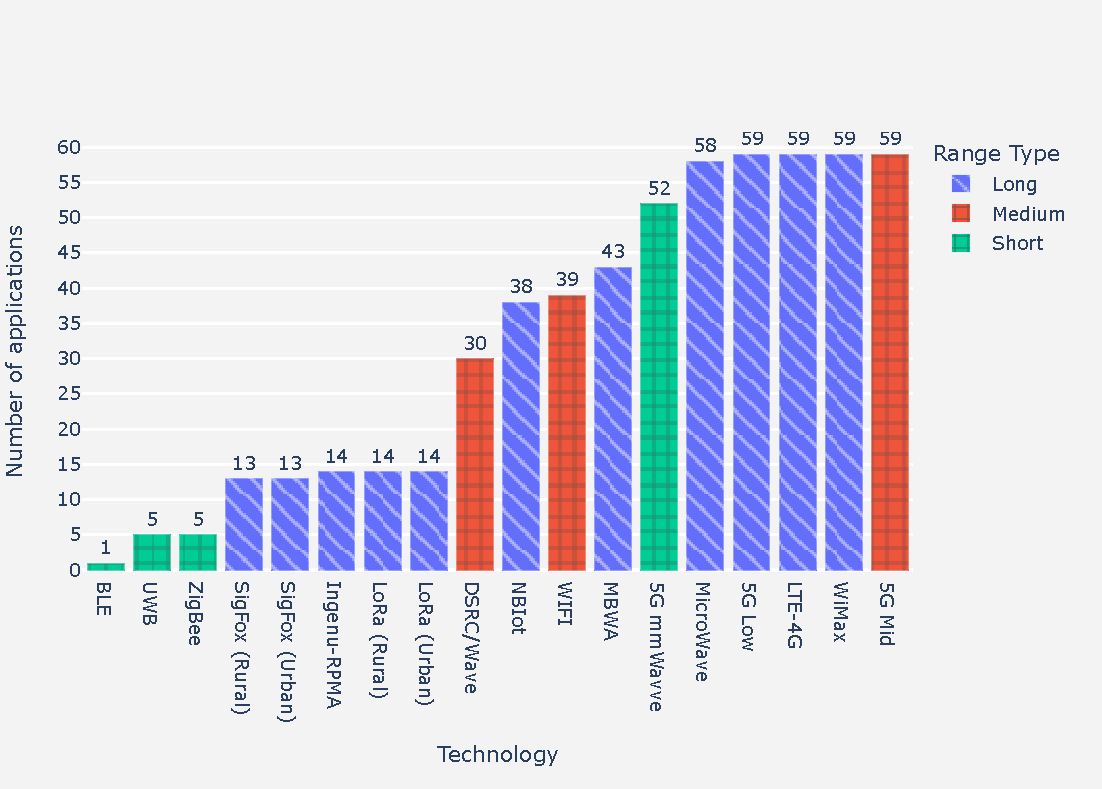
\includegraphics[width=0.9\textwidth]{bar_plot.pdf}
    \caption{Number of specific application usable by technologies.}
    \label{fig:barplot}
  \end{center}
\end{figure}

The result of the mapping can be illustrated in several ways. First, Figure~\ref{fig:boxplot} shows the distributions of the number of technologies that can be used by category, where categories are non-exclusive. It is clear that security and efficiency applications have the lowest number of suitable technologies, which is expected since they have some of the most demanding requirements, especially in terms of latency. Looking at Table~\ref{fig:techandapplong} and~\ref{fig:techandapplong2}, the technologies that can satisfy these categories are mainly 5G, 4G, NBIoT and WiMax. At the other end, the shared transport category has the most technology available to support its applications.

Second, Table~\ref{fig:table_techno} presents the proportion of applications in each category that are supported by each technology. Such a visualization provides more details than Figure~\ref{fig:boxplot} and helps identify quickly which technology to choose for a categoy or several categories of applications, apart from the all-purpose cellular technologies. 

Third, Figure~\ref{fig:barplot} represents the number of applications supported by each technology, ie.\ for which each technology can be used. Again, the clear ``winners'' are 5G and 4G technologies, along with WiMax, which can all be used for all the applications. 
%, 5G-Mid coming a close second, with the \acrfull{PCW} application being an exception because of its requirement of very low latency.
The figure also demonstrates the correlation between the range of the technology and the number of supported applications, in particular with the short range communication technologies supporting the smalled number of applications, between 1 and only 5. 5G technologies are exceptions since the short and medium range versions are expected to support all application in dense deployments to support the other uses of cellular networks. 

%{\bf NS: ajouter quelques commentaires si on ajoute le tableau des pourcentages d'applications supportees par categorie\\ conclure sur le fait que 5G est polyvalente, mais que 4G/LTE fait deja la job?} {\bf HB: Ajout de suite}
%It should be noted that WiMax and cellular technologies, with the exception of 5G mmWave, have entire uses in each category of applications.
%As can be seen in Figure ~\ref{fig:boxplot}, the Shared Transport category is the one that allows the most technologies to be developed for all of these applications. However, the categories containing the applications requiring demanding KPIs generates a reduction of their percentages of usable applications, like Entertainment applications. Finally, the short range technologies are those with the lowest percentage of applications in all categories. 

%According to the results of this taxonomy, 5G technologies merge with all the requirements of communicating applications for any category. However, based on our research, it appears that the previous generation, 4G, can also meet these requirements as well as WiMax technologies. These results also reveal that there are also a plurality of technological alternatives to the implementation of CA. However, the greater the requirements, the narrower the scope. 

\begin{landscape}
\begin{table}[ht!]
  \begin{center}
    \caption{Proportion of the applications in each category supported by each communication technology.}
    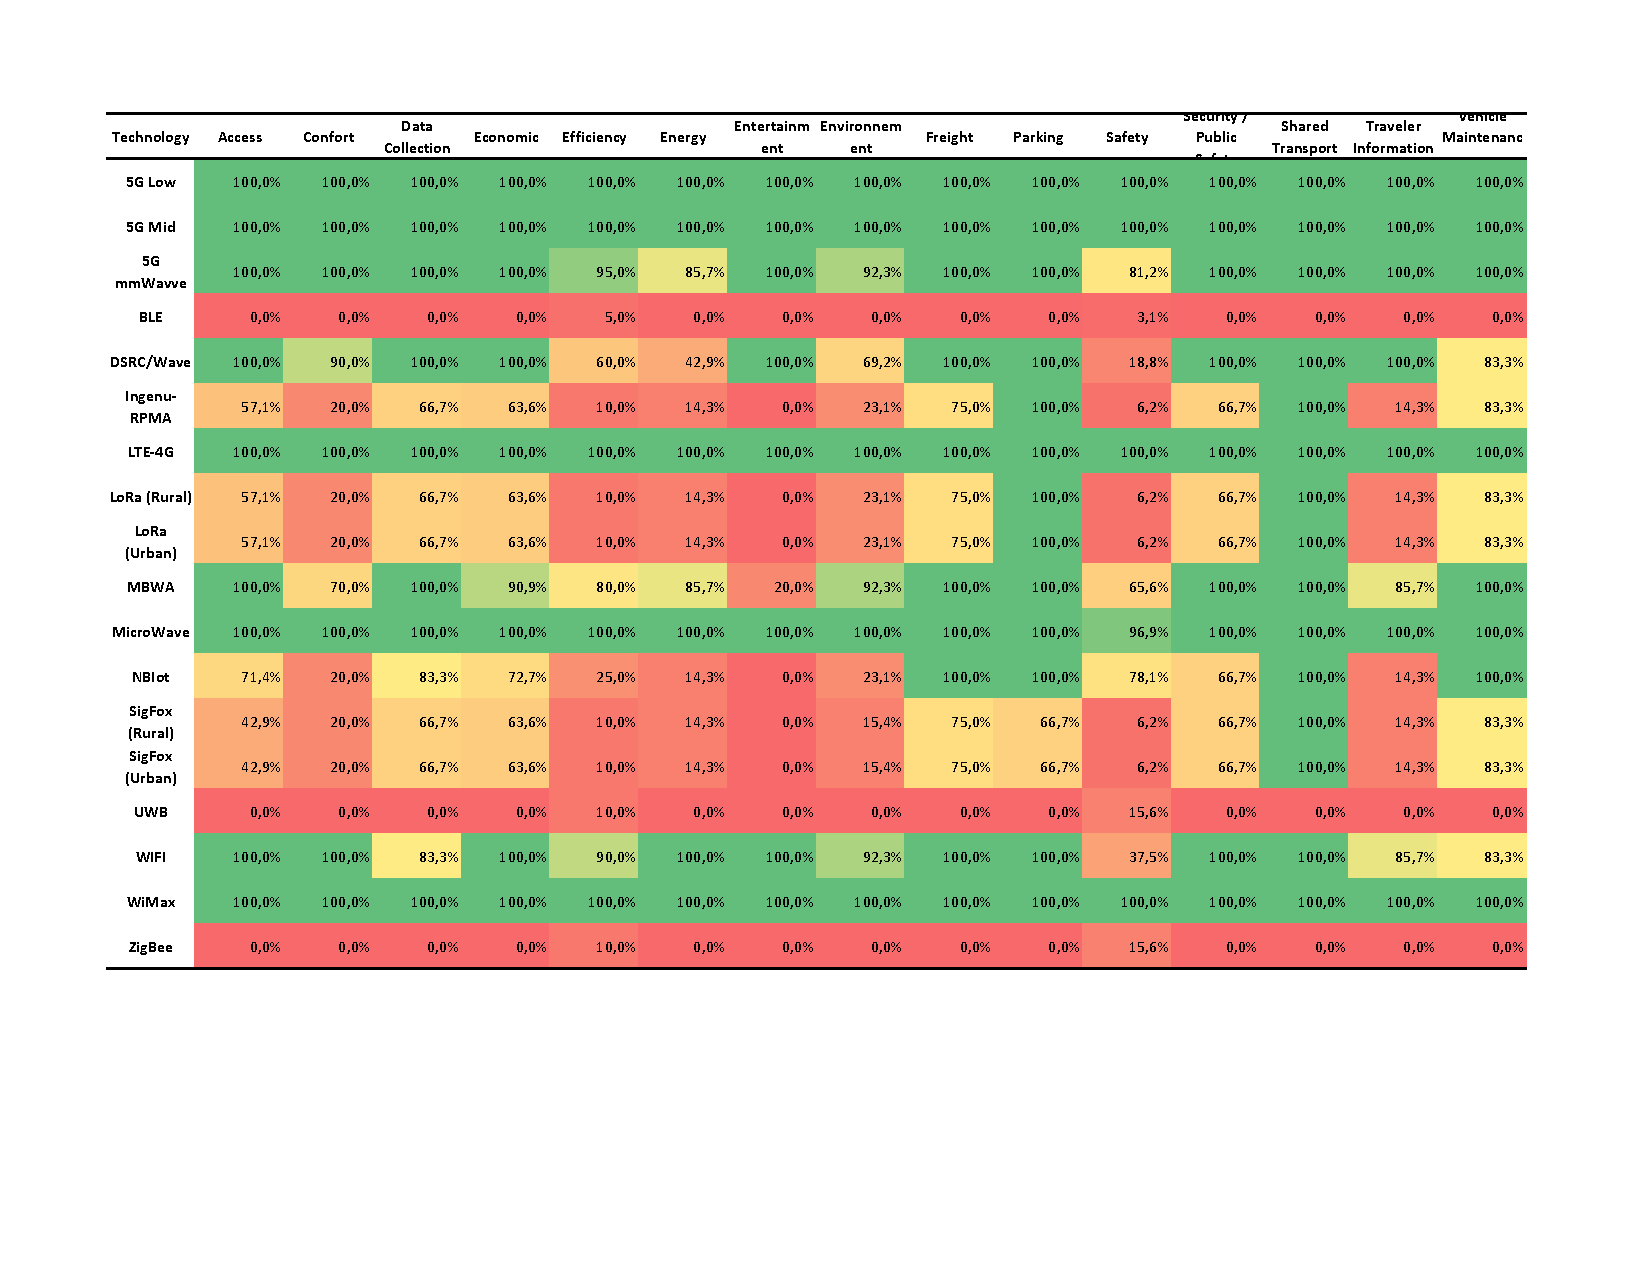
\includegraphics[width=1.5\textwidth]{tableau_percentage.pdf}
    \label{fig:table_techno}
  \end{center}
\end{table}
\end{landscape}




%By dint of the data we have collected, for this application it will seem that 5G is the most favorable for the good implementation of this application. With the following performance. Fig\ref{fig:techandapplong}\ref{fig:techandappmedium}\ref{fig:techandappshort}
%We can therefore make this deduction for other applications and thus assimilate the technologies that can be used for each application. 

